% TRASH
% This is kept only for future reference

The statistics of quantum particles, essentially the corresponding exchange operator, can be modeled by changing the kinetic energy operator from
\begin{equation}
 \widehat{T} = ∑_{j=1}^n -∇ⱼ^2
\end{equation}
to
\begin{equation}
 \widehat{T}_A = ∑_{j=1}^n \left( -i ∇ⱼ + Aⱼ \right)^2,
\end{equation}
where $A$ is a connection one-form on the bundle of which the wave function is a section. See \cref{rem:fiber bundels}. The following example illustrates this.

\begin{example}
  TODO skriv ner fr. tidigare anteckningar: Två abelska anyoner. Connection $Aⱼ = α ∑_{j \ne k} \frac{(xⱼ - xₖ)^\perp}{|xⱼ-xₖ|^2}$.
\end{example}

FRÅGA: Finns det enkelt exempel på connection som ger icke-abelskta anyoner?

This principle allows us to easier work with anyonic wave function with general with exchange operator $U$,
\begin{equation}
  ψ_A(-x_{jk}^\text{rel}, x_{jk}^\text{cm}) = U ψ_A(x_{jk}^\text{rel}, x_{jk}^\text{cm}),
\end{equation}
by instead considering symmetric wave functions, i.e.\
\begin{equation}
  ψ_0(-x_{jk}^\text{rel}, x_{jk}^\text{cm}) = ψ_0(x_{jk}^\text{rel}, x_{jk}^\text{cm}),
\end{equation}
and instead introducing a connection $A$ that implements the exchange operator $U$. That is, replacing $-i∇ⱼ$ with $-i∇ⱼ+Aⱼ$.



FRÅGA: Vad händer med parallelogram-identiteten? Är det varför man istället jobbar med $ψ_A$ så länge som möjligt? Nästa steg, ta uttrycket
\begin{equation}
  ∫_{ℝᵈ} \left|∇_{x_{jk}^\text{rel}}u\right|^2  2 dx_{jk}^\text{rel}
\end{equation}
från beviset av satsen ovan, låt $d = 2$ för att få anyoner, och skriv om det som i anteckningarna från tidigare. Hur går man från denna integral till att bara titta på övere halvplanet? För att tillåta $ψ$ att vara problematisk ($ψ_A$). Sen byter man variabel ($x_{jk}^\text{rel} = (r, φ)$), sen har man
\begin{equation}
  ∫_{ℝ^2} \left|∇_{x_{jk}^\text{rel}}u\right|^2  2 dx_{jk}^\text{rel} =
  ∫_{r=0}^\infty ∫_{φ=0}^\pi \left|\partial_r ψ\right|^2 + \frac{1}{r^2} \left|\partial_\varphiψ \right|^2  2 dr d\varphi
\end{equation}
sen återgår vi till $ψ_A$ (här är jag förvirrad igen, exakt när och varför byter vi mellan att lägga anyoniciteten på vågfunktionen eller $∇$?), och slutligen tittar vi bara på
\begin{equation}
  ∫_{φ=0}^π \left|\partial_\varphiψ_A \right|^2 dr
\end{equation}
vilket ger att det är spektrumet till $U$ som är relevant. Använd Poincare olikheten (5.16) \cite{methmmp}? Vilket är baktanken till resten av uppsatsen.

TODO: Delar av diskussionen från gamla versionen nedan ska tas med, så som annulus, visa resultatet för abelska anyoner, och diskussionen om icke-abelska.

% To sum up, the kinetic energy operator can be written as
% \begin{equation}
%   \widehat{T} = ∑_{j=1}^n \left( -i ∇ⱼ^\mathbf{A} \right)^2
% \end{equation}
% for some connection $\mathbf{A}$ which implements the statistics, i.e.\ a simple exchange gives rise to a given exchange operator.




















\hrule

\textbf{Det gammla:}

\section{Preliminaries}

Consider $n$ anyons in $ℝ^2$, with coordinate $x₁, …, x_n$. This collection of anyons are described by an $n$-particle wave function $ψ ∈ L^2(ℝ^{2n})$, i.e.\ a square-integrable complex-valued function on $ℝ^{2n}$. The kinetic energy $T$ of this system is by definition
\begin{equation} % \cite{lundholm-solovej} (3)
  T ≔ ∑_{j=1}^n ∫_{ℝ^{2n}} |∇ⱼ ψ|^2 dx
\end{equation}
where $\Deltaⱼ$ acts on $xⱼ$.
In order to give bounds for the kinetic energy we shall determine the kinetic energy for pairs of anyons, by factoring out the dynamics of two anyons from the system of $n$ anyons.

Among the $n$ anyons, let all except two of them be fixed. Let $xⱼ, xₖ ∈ ℝ^2$ denote the coordinates for the two free anyons and define
\begin{equation}
  x_\text{cm} = \frac{1}{2}(xⱼ + xₖ), \quad
  x_\text{rel} = \frac{1}{2}(xⱼ - xₖ).
\end{equation}
Consider a frame of reference where the center of mass is at the origin, i.e.\ $x_\text{cm} = 0$. Let $(r, \varphi)$ be the polar coordinates for the relative coordinates $x_\text{rel}$. The $n$-particle wave function can thus be parameterized as
\begin{equation}
  ψ = ψ(x', r, \varphi),
\end{equation}
where $x'$ is the coordinates for the anyons that we considered to be fixed. If we also freeze out the radial dependence by fixing $r$, we factor out the angle-dependence from the wave function and write
\begin{equation}
  ψ(\varphi) ≔ ψ(x', r, \varphi).
\end{equation}

We shall consider the angular dynamics of the two free anyons. As the free anyons circle each other, i.e.\ as $\varphi$ increases from $0$ to $π$, a number of fixed anyons may be enclosed. As we shall see, the number of encircled anyons will play a crucial role, therefore we separate the state space $ℝ^2$ as follows.

Separate the state space into open annuli (regions between two concentric circles) such that none of the fixed $n-2$ anyons are at the interior of an annulus, cf.\ \cref{fig:annuli}. This gives a separation of $ℝ^2$ into regions with increasing number $p$ of the $n-2$ fixed anyons. More explicitly, each annulus is centered in $x_\text{cm}$. Furthermore, let $r₁ \le r_2 \le … \le r_{n-2}$ be the radii of the $n-2$ fixed anyons. The innermost annulus is an open disc (degenerate annulus) with radius $r₁$, the second innermost annulus is the region between circles of radius $r₁$ and $r_2$, etc. Note that the circles with radii $r₁, r_2, …, r_{n-2}$ are not contained in any annuli, since the anyons cannot pass through each other, and we are considering angular motion. If the radii of two fixed anyons coincide, then there is clearly no annulus separating them.

\begin{figure}[h]
  \centering
  \begin{tikzpicture}
    \draw[->] (-3.75,0) -- (3.75,0) node[below] {$x$};
    \draw[->] (0,-3.75) -- (0,3.75) node[right] {$y$};
    \draw (0,0) circle (1.25);
    \draw (0,0) circle (2);
    \draw (0,0) circle (3);
    \node at (0.5, 0.35) {$p = 0$};
    \node at (0.5, 1.5) {$p = 1$};
    \node at (0.5, 2.375) {$p = 2$};
    \node at (0.5, 3.25) {$p = 3$};
    \node[font=\Large] at ({1.25*cos(220)}, {1.25*sin(220)}) {$\bullet$};
    \node[font=\Large] at ({2*cos(130)}, {2*sin(130)}) {$\bullet$};
    \node[font=\Large] at ({3*cos(-55)}, {3*sin(-55)}) {$\bullet$};
    \node at (1.5, -0.2) {$r₁$};
    \node at (2.25, -0.2) {$r_2$};
    \node at (3.25, -0.2) {$r_3$};
  \end{tikzpicture}
  \caption{Illustration of annuli separating $ℝ^2$ into regions with increasing number $p$ of contained anyons. A blob ($\bullet$) denotes a fixed anyon. In each annulus, exchange of the two free anyons, i.e.\ as $\varphi$ increases from $0$ to $\pi$, a given number $p$ of fixed anyons will be enclosed.}
  \label{fig:annuli}
\end{figure}

In the general case, exchange of a pair of anyons introduces an anyonic phase $U_p ∈ U(n)$ as discussed in \cref{chap:how anyons arise}. The exchange operator $U_p$ may depend on the number $p$ of anyons that get encircled in the exchange loop. With the wave function $ψ = ψ(\varphi)$ parameterized by the relative angular coordinate, we thus get the boundary condition
% \begin{alignat*}{3}
%   ψ(-r) &= U_p ψ(r), && \quad \text{at the innermost annulus, containing no fixed anyons} \\
%   ψ(-r) &= U_p ψ(r), && \quad \text{at an annulus enclosing $p$ fixed anyons.}
% \end{alignat*}
% \begin{equation*}
%   ψ(-r) = U_p ψ(r)
% \end{equation*}
% at an annulus enclosing $p$ anyons.
\begin{equation}\label{U_p boundary condition}
  ψ(π) = U_p ψ(0).
\end{equation}
This essentially alters the geometry of the space, splitting it in half. It suffices to consider the region $0 \le \varphi \le π$, i.e.\ it suffices to consider half annuli.

We have set out to estimate the energy of the system, this amounts to solving the Schrödinger equation, in particular solving for the lowest energy $λ$,
\begin{equation}
  H ψ = λ ψ
\end{equation}
where $H = -∇^2 = -\frac{\partial^2}{\partial\varphi^2}$ is the Hamiltonian of the system.
So far we have just one boundary condition, \cref{U_p boundary condition}, while the Schrödinger equation is a second order differential equation, requiring two boundary conditions to give a unique solution.
However, since we are primarily interested the energies of the system, it suffices to compute the spectrum of $H$. With this in mind, we write the Hamiltonian $H = -∇^2$ as a square $H = D^2$, where
\begin{equation}
  D = -i\partial_\varphi, \quad 0 \le \varphi \le π, \text{ subject to boundary conditions given by $U_p$,}
\end{equation}
and use the spectral theorem to compute the spectrum of $H$ as the squared spectrum of $D$, i.e.
\begin{equation}
  σ(H) = \{λ^2 : λ ∈ σ(D)\}.
\end{equation}
Similarly, we have that the ground state energy is the infimum of $σ(H)$, i.e.
\begin{equation}
  λ_0 = \inf σ(H) = \inf \{λ^2 : λ ∈ σ(D)\}.
\end{equation}
The spectrum of $D$ is straight forward to compute and we present the result as a lemma.

\begin{lemma}
  % Consider a pair of anyons subject to the boundary condition \cref{U_p boundary condition}.
  The eigenfunctions $u$ and eigenvalues $λ$ of $D$ are such that
  \begin{equation}
    D u = λ u \quad \iff \quad -iu'(\varphi) = λ u(\varphi),
  \end{equation}
  having general solution
  \begin{equation}
    u(\varphi) = C e^{iλ\varphi}
  \end{equation}
  for some constant $C ∈ \mathbb{C}^n$.
\end{lemma}

We seek an expression for the spectrum of $D$, the above lemma and the boundary condition \cref{U_p boundary condition} gives
\begin{equation}
  u(π) = U_p u(0) \implies
  C e^{iλπ} = U_p C,
\end{equation}
that is, $e^{iλπ}$ is an eigenvalues of $U_p$. We have the following result.

\begin{lemma}\label{D spectrum}
  The spectrum of $D$ (and by extension the spectrum of $H$) is given by
  \begin{equation}
    σ(D) = \big\{λ : e^{iλπ} \text{ is an eigenvalue of } U_p\big\}.
  \end{equation}
\end{lemma}

\begin{remark}
  Recall that $U_p$ is unitary, so all eigenvalues of $U_p$ are on the complex unit circle. Hence, each eigenvalue $e^{iλπ}$ of $U_p$ with $0 \le λ < 2$, gives a family of possible energy levels $\big\{(λ + 2n)^2 \mid n ∈ ℤ\big\}$ to the system.
\end{remark}





\section{Abelian anyons}\label{sec:statistical repulsion abelian ayons}

Although non-abelian anyons are the main focus of this thesis, we give a quick overview of the case of abelian anyons. For more details, see \cite{lundholm-solovej}
% In full generality for abelian anyons we have the following.

Abelian anyons are characterized by the fact that the exchange operator is one-dimensional, i.e.\ an element of $U(1)$, hence it is of the form $e^{iα\pi}$. Take this to be $U_0$, i.e.\ simple exchange of a pair of abelian anyons, with the exchange loop enclosing no other anyons. It is then easy to realize that
\begin{align}\label{eq:abelian Up}
  U_p = e^{iα(1+2p)π}
\end{align}
because the left anyon performs an exchange with the $p$ inner anyons, likewise for the right anyon, finally the two anyons undergoing exchange are exchanged with each other, resulting in $1+2p$ exchanges of $α$-type anyons, as illustrated in \cref{fig:abelian Up}.

\begin{figure}[h]
  \centering
  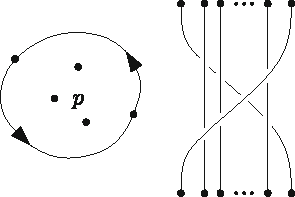
\includegraphics{img/interchange_loop_p.pdf}
  \caption{Exchange of a pair of abelian $α$ anyons around $p$ fixed $α$ anyons. Figure taken from \cite{lundholm-solovej}.}
  \label{fig:abelian Up}
\end{figure}


\begin{proposition}[Ground state energy for a pair of abelian anyons]
  Consider a pair of abelian anyons with anyonic phase $α$ enclosing $p$ fixed anyons (also with anyonic phase $α$).
  The ground state energy is bound from below by
    \begin{gather*}
      \inf_{p,q∈ℤ} \left(α(1+2p)+2q\right)^2 =\\
      = \begin{cases}
        \frac{1}{ν^2}, & \text{if $α = \frac{μ}{ν}$ with $μ ∈ ℤ, ν ∈ ℕ_+$ relatively prime and $μ$ odd}, \\
        0, & \text{otherwise}
      \end{cases}
    \end{gather*}
\end{proposition}

\begin{proof}
  By \cref{eq:abelian Up} we have the anyonic exchange operator as
  \begin{equation}
    U_p = e^{iα(1+2p)π}.
  \end{equation}
  By \cref{D spectrum} we have that the boundary condition gives
  \begin{equation}
    \begin{aligned}
      &u(π) = e^{iα(1+2p)π} u(0) \\
      \iff\;\; &e^{iλ π} = e^{iα(1+2p)π} \\
      \iff\;\; &λ = α(1+2p) + 2q, \quad q ∈ ℤ.
    \end{aligned}
  \end{equation}
  Thus we see that the spectrum for $D$ and $H = D^2$, respectively, is
  \begin{equation}
    \begin{aligned}
      σ(D) &= \{ α(1+2p) + 2q : q ∈ ℤ\}, \\
      σ(H) &= \{ (α(1+2p) + 2q)^2 : q ∈ ℤ\}.
    \end{aligned}
  \end{equation}
  Hence, the energy $λ^2$ is minimized for
  \begin{equation}
    E_0 = \inf_{p,q∈ℤ} (α(1+2p)+2q)^2.
  \end{equation}
  A number-theoretic result, found as proposition 5 in \cite{lundholm-solovej}, shows that this can be written as
  \begin{equation}
    E_0 =
    \begin{cases}
      \frac{1}{ν^2}, & \text{if $α = \frac{μ}{ν}$ with $μ ∈ ℤ, ν ∈ ℕ_+$ relatively prime and $μ$ odd}, \\
      0, & \text{otherwise}.
    \end{cases}
  \end{equation}
\end{proof}

From this we have an immediate corollary for bosons ($α = 0$) and fermions ($α = 1$).

\begin{corollary}
  With $α = 0$, the anyonic phase reads
  \begin{equation}
    U_p = e^{iα(1+2p)π} = 1
  \end{equation}
  for all $p$, i.e.\ bosons do not ``see'' each other, and they have a zero ground state energy.

  With $α = 1$, the anyonic phase reads
  \begin{equation}
    U_p = e^{iα(1+2p)π} = e^{i(1+2p)π},
  \end{equation}
  giving us the boundary condition
  \begin{equation}
    e^{iλ π} = e^{i(1+2p)π} \iff λ = 1 + 2p + 2q, \quad q ∈ ℤ
  \end{equation}
  Since $p$ is an integer, this shows that also fermions do not ``see'' the enclosed $p$ anyons.
  However, the anyons in the pair do ``see'' each other, in the sense that their wave function changes sign after they have been exchanged, as expected. Finally, this also shows that fermions have a non-zero ground state energy $E_0 = 1$.
\end{corollary}












\section{Non-abelian anyons}

Consider the same setting as above, with the distinction that the anyons are now non-abelian. That is, consider a pair of non-abelian anyons, with wave function $ψ ∈ L^2(ℝ; \mathbb{C}^n)$ parameterized by the relative angle $\varphi$, such that the pair of anyons encloses $p$ fixed anyons as $\varphi$ increases from $0$ to $π$, giving rise to an anyonic phase $U_p ∈ U(n)$.

% From \cref{D spectrum} the boundary condition reads
% \begin{equation}
%   u(π) = U_p u(0) \iff C e^{iλπ} = U_p C.
% \end{equation}
% This is precisely the condition that $e^{iλπ}$ is an eigenvalue of $U_p$.


% \hrule

% Consider first the case $n=2$, then $U_p ∈ U(2)$ can be parameterized as follows.

% \begin{lemma}[Characterization of $U(2)$ matrices]
%   Let $U ∈ U(2)$, then
%   \begin{equation}
%     U = \begin{pmatrix} a & b \\ -e^{i\thetaπ}\overline{b} & e^{i\thetaπ} \overline{a} \end{pmatrix}, \quad \operatorname{det} U = e^{i\thetaπ}.
%   \end{equation}
%   for $a,b,\theta ∈ ℝ$ such that $\abs{a}^2 + \abs{b}^2 = 1$ and $0 \le \theta < 2$.
%   The parameter $\theta$ corresponds to the abelian phase in the factorization $U(2) = U(1)\times SU(2)$, where $\theta = 0$ gives $SU(2)$.
% \end{lemma}

% \hrule

A standard characterization of unitary matrices is as follows.

\begin{lemma}
  Let $U ∈ U(n)$, the $n$ eigenvalues (counted with multiplicity) of $U$ are on the form $e^{iβⱼπ}$ for $j = 1,2,…,n$. Furthermore, $e^{iα\pi}$ where $α = \frac{1}{n}∑ⱼ βⱼ$ is referred to as the abelian phase of $U_p$. It is the abelian part in the factorization of $U(n) = U(1) \times SU(n)$. Note that if $\det U = e^{iθπ}$ we have $α = θ/n$.
\end{lemma}

\begin{proof}
  We only show the $U(n) = U(1) \times SU(n)$ decomposition.
  Rewrite $U$ as $U = e^{iα}\left( e^{-iα} U \right)$ where $e^{iα}$ is the abelian part and $e^{-iα} U$ is the $SU(n)$ part. It suffices to show that $\det \left( e^{-iαπ} U \right) = 1$,
  \begin{equation}
    \begin{aligned}
      \det \left( e^{-iαπ} U \right)
      &= \left(e^{-iαπ}\right)^n e^{i\left(∑ⱼ βⱼ\right)π} \\
      &= \left(e^{-i\left(∑ⱼ βⱼ\right)π/n}\right)^n e^{i\left(∑ⱼ βⱼ\right)π} = 1.
    \end{aligned}
  \end{equation}
  On the other hand, $1 = \det \left( e^{-iαπ} U \right) = e^{-iαπn} e^{iθπ} = e^{i(-αn+θ)π}$, thus $α = θ/n$ (mod $2$).
\end{proof}

Next, we show that the abelian phase shifts the eigenvalues uniformly along the complex unit circle.

\begin{proposition}
  Consider non-abelian anyons with arbitrary (unitary) $U_p ∈ U(n)$ exchange operator. The abelian part of the non-abelian anyonic phase $U_p$ can always be chosen so that the ground state has zero energy.
\end{proposition}

\begin{proof}
  By changing the abelian phase, each eigenvalue is shifted. This is obvious if we diagonalize $U_p$. In particular, adding $-βⱼ$ to the abelian phase, the $j$:th eigenvalue is shifted to $e^{i(βⱼ-βⱼ)} = 1$, corresponding to zero energy.
\end{proof}

% From this, the abelian part $e^{iαπ}$ of the anyonic phase $U_p ∈ U(n)$ can be seen as a shift of the eigenvalues $e^{iλπ}$ of $U_p$ along the complex unit circle, where $λ^2$ gives the energy of the system, as shown in figure \cref{fig: abelian phase shift}.

% \begin{figure}
%   \centering
%   ∈cludegraphics[width=0.5\linewidth]{img/abelian-phase-shift.jpg}
%   \caption{The shift of energy levels due to an abelian phase $α$ TODO it says theta.}
%   \label{fig: abelian phase shift}
% \end{figure}

As we shall see in the following chapter, the exchange operator $U_p$ has a rather involved dependence on the particular type of non-abelian anyons that are considered. In order to characterize the energy bound, via the eigenvalues of $U_p$, we must first dive into the framework of abstract anyon models in order to characterize $U_p$.
